% Provenance (never printed): see sources/outline_sources.md (Year 1: field
% notebook, compass-clinometer, hand lens, sampling, polarising microscope and
% thin sections, safety). The readings of the Varden east limb are simulated
% in figdata/bachelor-1/attitude_stats.py (seed 83, errors of 3 degrees);
% problem values in the Book 3 scratch calculator calc/ch06.py.
\chapter{Métodos de campo e de laboratório I}\label{ch:b1:field-lab-methods-1}

Uma geóloga que mapeia as Colinas de Varden leva pouca coisa: um caderno, um lápis, um receptor de satélite, uma bússola-clinômetro, uma lupa e alguns sacos de amostras. Com eles ela fixa onde está, mede a \omterm{def:b1:geological-maps:attitude}{atitude} dos estratos, dá nome às rochas e traz as amostras que o laboratório vai cortar, desbastar e observar ao microscópio. Cada número dos capítulos anteriores --- uma \omterm{def:b1:geological-maps:attitude}{atitude} num mapa, um \omterm{def:b1:geological-maps:attitude}{mergulho} numa seção --- começou como uma leitura desse tipo, com seu próprio erro. Este capítulo descreve como os profissionais fazem essas observações e como leituras repetidas são calculadas em média e sua dispersão transformada em incerteza. Ele termina com uma temporada de leituras no flanco leste do \omterm{def:b1:geological-maps:fold}{anticlinal} de Varden.

\begin{recall}
A \omterm{def:b1:geological-maps:attitude}{atitude} de um plano se escreve \omterm{def:b1:geological-maps:attitude}{sentido de mergulho}/\omterm{def:b1:geological-maps:attitude}{mergulho}, como $081/12$, ou como uma \omterm{def:b1:geological-maps:attitude}{direção} pela regra da mão direita com um \omterm{def:b1:geological-maps:attitude}{mergulho} (\cref{ch:b1:geological-maps}). A declinação magnética é o ângulo entre o norte geográfico e a \omterm{def:b1:geological-maps:attitude}{direção} para a qual aponta a agulha de uma bússola (física, 11º ano). Os minerais são reconhecidos na mão pelo brilho, pela clivagem, pela dureza e pela cor (Livro 2, 11º ano). A média e o desvio padrão de um conjunto de números resumem o seu centro e a sua dispersão (matemática).
\end{recall}

\section{O caderno e o mapa}

\begin{definition}[Estação de campo, caderneta de campo]\label{def:b1:field-lab-methods-1:station}
Uma \emph{estação de campo}\index{estação de campo} é um lugar numerado onde um geólogo faz e registra observações: sua posição, as rochas vistas, a sua \omterm{def:b1:geological-maps:attitude}{atitude} e as amostras colhidas. A \emph{caderneta de campo}\index{caderneta de campo} é o registro encadernado das estações, na ordem em que foram visitadas, com seus números, esboços e medidas, anotados no local.
\end{definition}

A caderneta é o registro primário: o que não é anotado na estação se perde, e um mapa desenhado à noite só vale tanto quanto as anotações que o sustentam. Cada estação tem um número que aparece no mapa de campo, na caderneta e em cada saco de amostra recolhido ali. Um esboço mostra o que uma lista de números não consegue --- como duas unidades se encontram, para que lado estão as camadas mais novas, onde uma leitura foi feita numa superfície dobrada --- e registra a sua escala e orientação. Fatos e interpretações são mantidos separados: ``calcário sobre folhelho, contato nítido'' é uma observação; ``\omterm{def:b1:cross-sections:unconformity}{discordância}'' é uma inferência, escrita como tal.

\begin{inthefield}[Um dia de mapeamento]
% ledger: gps:smartphone-accuracy, gps:high-end
\begin{minipage}[t]{0.58\linewidth}\vspace{0pt}
Um geólogo que mapeia planeja um caminhamento transversal à \omterm{def:b1:geological-maps:attitude}{direção}, de modo a encontrar cada unidade em sequência, e para em cada contato, mudança de rocha ou superfície mensurável que aparece. Em cada estação ela anota o número e a posição, esboça o que vê, mede \omterm{def:b1:geological-maps:attitude}{atitudes} e registra as amostras. As posições vêm de um receptor de satélite: um receptor comum, como o de um smartphone, tem precisão típica de cerca de \qty{4.9}{m} a céu aberto, pior perto de paredões e árvores, enquanto receptores de levantamento de dupla frequência ou com serviços de correção chegam a poucos centímetros. Na escala 1:10\,000, \qty{4.9}{m} são meio milímetro: um receptor comum basta para o mapeamento, mas não para medir o movimento lento do terreno (\cref{ch:b1:plate-kinematics}).
\end{minipage}\hfill
\begin{minipage}[t]{0.39\linewidth}\vspace{0pt}
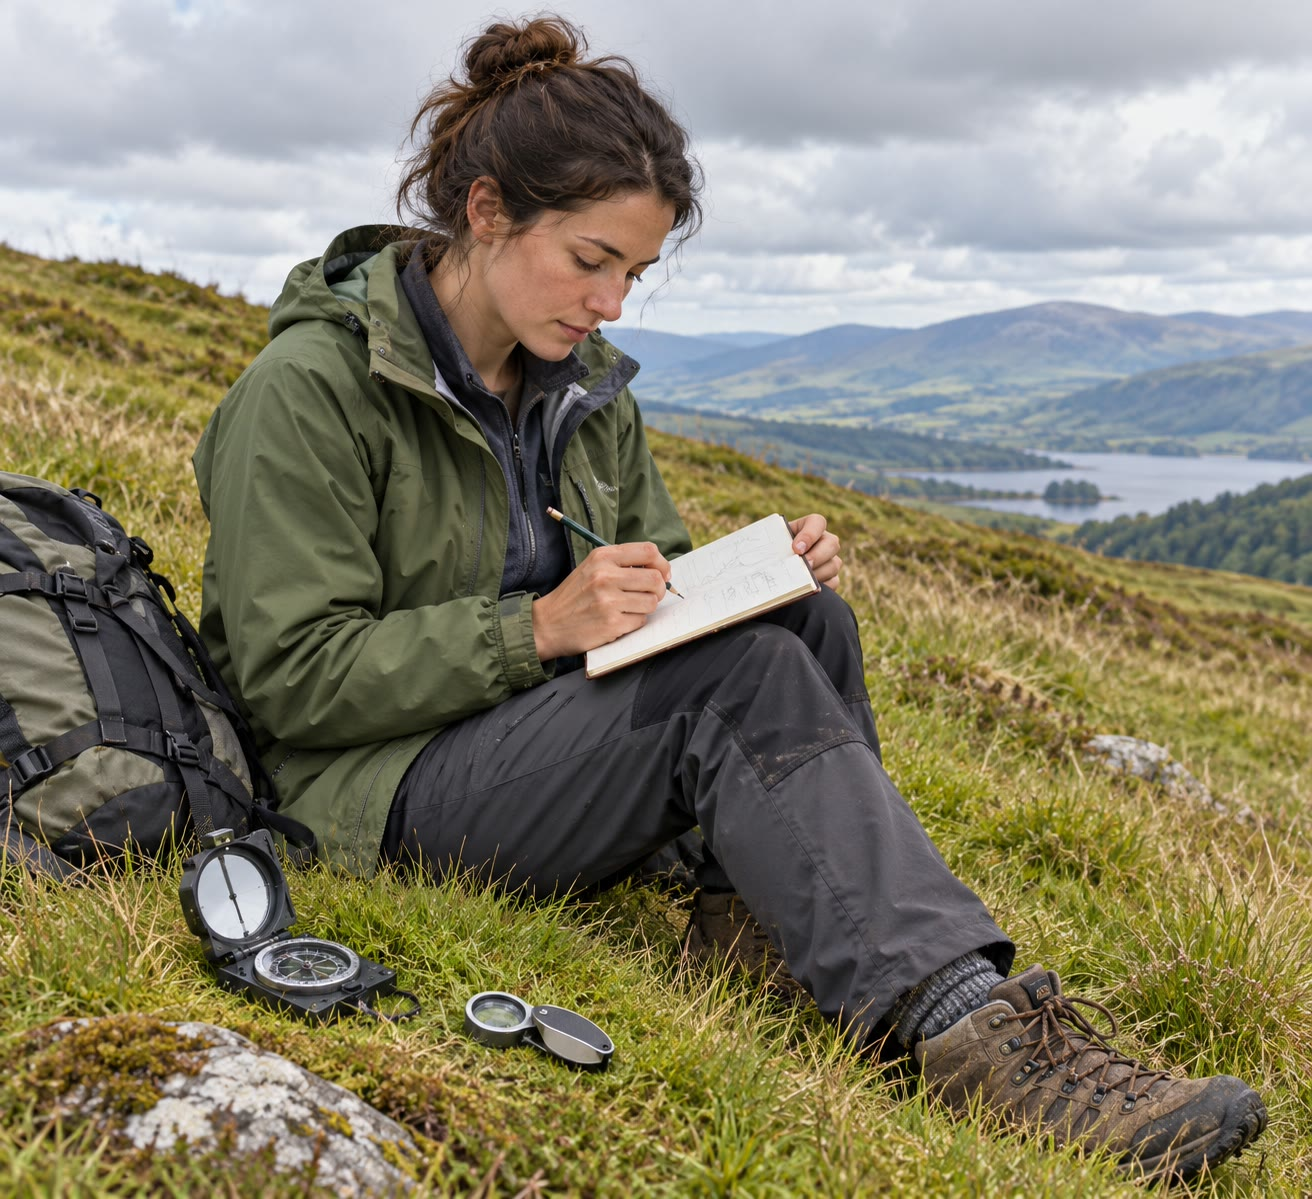
\includegraphics[width=\linewidth]{images/book3/ai/b1-field-notebook.jpg}
\end{minipage}
\end{inthefield}

\section{Medindo orientações}

A \omterm{def:b1:geological-maps:attitude}{atitude} de um plano --- um estrato, uma falha, uma junta --- é medida com uma bússola-clinômetro: uma bússola magnética para ler \omterm{def:b1:spherical-astronomy:horizontal}{azimutes}, e um pêndulo ou um nível para ler ângulos a partir da horizontal. Sua borda é apoiada ao longo da \omterm{def:b1:geological-maps:attitude}{direção} da superfície para ler a \omterm{def:b1:geological-maps:attitude}{direção}, ou o instrumento é posto sobre a superfície ao longo da sua linha de maior declive para ler o \omterm{def:b1:geological-maps:attitude}{mergulho} e, a partir do \omterm{def:b1:spherical-astronomy:horizontal}{azimute} dessa linha, o \omterm{def:b1:geological-maps:attitude}{sentido de mergulho}.

\begin{omfigure}
\begin{tikzpicture}[font=\scriptsize]
% (a) plan view
\begin{scope}
\fill[icsJurassic!25] (0,0) -- (3.6,0.5) -- (3.9,2.9) -- (0.3,2.4) -- cycle;
\draw (0,0) -- (3.6,0.5) -- (3.9,2.9) -- (0.3,2.4) -- cycle;
\draw[omDef, thick] (0.4,1.55) -- (3.5,1.98);
\node[omDef, above, rotate=8, fill=icsJurassic!25, inner sep=1pt] at (0.95,1.65) {linha de direção};
% compass box laid along the strike line
\begin{scope}[shift={(2.5,1.84)}, rotate=8]
\draw[fill=white] (-0.6,0) rectangle (0.6,0.32);
\draw (0,0.16) circle (0.12);
\end{scope}
\draw[omThm, thick, -{Stealth[length=2mm]}] (1.6,1.71) -- (1.75,0.62);
\node[omThm, right, fill=icsJurassic!25, inner sep=1pt] at (1.78,0.85) {sentido de mergulho};
\node[below, align=center] at (1.95,-0.15) {(a) vista em planta: a borda da\\ bússola ao longo da direção};
\draw[->] (4.3,1.6) -- (4.3,2.4) node[above] {N};
\end{scope}
% (b) side view, vertical section along the dip direction
\begin{scope}[xshift=5.8cm]
\fill[icsJurassic!25] (0,1.6) -- (3.6,0.2) -- (3.6,-0.3) -- (0,-0.3) -- cycle;
\draw[thick] (0,1.6) -- (3.6,0.2);
% clinometer resting on the surface
\begin{scope}[shift={(2.5,0.6278)}, rotate=-21.25]
\draw[fill=white] (-0.75,0) rectangle (0.75,0.3);
\draw (0,0.15) circle (0.11);
\draw[black!70] (0,0.15) -- ++(-68.75:0.11);
\end{scope}
% dip angle at the lower end of the surface
\coordinate (P) at (0.7,1.3278);
\draw[black!60] (P) -- ++(1.6,0) node[right] {horizontal};
\draw[omThm] ($(P)+(1.1,0)$) arc[start angle=0, end angle=-21.25, radius=1.1];
\node[omThm] at ($(P)+(0.9,-0.15)$) {$\delta$};
\node[below, align=center] at (1.8,-0.35) {(b) seção ao longo do sentido de mergulho:\\ o clinômetro sobre a linha mais íngreme};
\end{scope}
\end{tikzpicture}

{\small Medindo uma \omterm{def:b1:geological-maps:attitude}{atitude} (esquemático). (a) A borda da bússola apoiada horizontalmente sobre o estrato dá a \omterm{def:b1:geological-maps:attitude}{direção}; o \omterm{def:b1:geological-maps:attitude}{sentido de mergulho} é perpendicular a ela, descendo pelo estrato. (b) Posto sobre a borda, ao longo da linha mais íngreme, o clinômetro dá o \omterm{def:b1:geological-maps:attitude}{mergulho} $\delta$.}
\end{omfigure}

Uma linha --- o eixo de uma \omterm{def:b1:geological-maps:fold}{dobra}, um risco numa superfície de falha, o eixo longo de seixos --- tem uma orientação própria.

\begin{definition}[Rumo e caimento]\label{def:b1:field-lab-methods-1:trend-plunge}
O \emph{rumo}\index{rumo (de uma linha)} de uma linha é o \omterm{def:b1:spherical-astronomy:horizontal}{azimute} da sua projeção horizontal, medido em direção à extremidade da linha que aponta para baixo. Seu \emph{caimento}\index{caimento} é o ângulo entre a linha e a horizontal, medido no plano vertical que a contém. Uma linha que cai \ang{20} em direção a \ang{015} escreve-se $20\to015$.
\end{definition}

Uma linha de \omterm{def:b1:field-lab-methods-1:trend-plunge}{rumo} $t$ e \omterm{def:b1:field-lab-methods-1:trend-plunge}{caimento} $p$ tem o vetor unitário para baixo $(\cos p\sin t, \cos p\cos t, -\sin p)$, em componentes leste, norte e cima; uma linha situada em um plano de \omterm{def:b1:geological-maps:attitude}{sentido de mergulho} $\alpha$ e \omterm{def:b1:geological-maps:attitude}{mergulho} $\delta$ cai pelo \omterm{def:b1:cross-sections:apparent-dip}{mergulho aparente} desse plano no plano vertical de \omterm{def:b1:spherical-astronomy:horizontal}{azimute} $t$, de modo que $\tan p = \tan\delta\cos(\alpha - t)$ (\cref{thm:b1:cross-sections:apparent-dip}).

\subsection{A declinação magnética}

Uma agulha de bússola aponta para o norte magnético, não para o norte geográfico; o ângulo entre os dois é a declinação magnética, contada como positiva quando o norte magnético está a leste do norte geográfico. Mapas e as \omterm{def:b1:geological-maps:attitude}{atitudes} deste livro usam \omterm{def:b1:spherical-astronomy:horizontal}{azimutes} geográficos.

\begin{method}[Correção de um azimute da bússola]\label{met:b1:field-lab-methods-1:declination}
\begin{enumerate}
  \item Encontre a declinação magnética $D$ para o lugar e a data, a partir de um modelo do campo terrestre (leste positivo, oeste negativo).
  \item Some a ela cada \omterm{def:b1:spherical-astronomy:horizontal}{azimute} lido na bússola: \omterm{def:b1:spherical-astronomy:horizontal}{azimute} geográfico $=$ \omterm{def:b1:spherical-astronomy:horizontal}{azimute} magnético $+ D$, módulo \ang{360}.
  \item Não altere \omterm{def:b1:geological-maps:attitude}{mergulhos} nem \omterm{def:b1:field-lab-methods-1:trend-plunge}{caimentos}: eles são medidos a partir da horizontal, pela gravidade, e não pela agulha.
\end{enumerate}
A maioria das bússolas de campo pode ser ajustada para somar $D$ mecanicamente; o ajuste, e o ano para o qual foi feito, são anotados na caderneta.
\end{method}

\begin{dated}{2026}
% ledger: noaa:wmm-edinburgh, noaa:wmm-reykjavik, noaa:wmm-anchorage, noaa:wmm-wellington
Em 1º de janeiro de 2026, o World Magnetic Model (versão 2025) dá a declinação magnética como \ang{-0.47} (oeste) em Edimburgo, variando \ang{+0.20} por ano; \ang{-11.28} em Reykjavik, variando \ang{+0.30} por ano; \ang{+14.20} (leste) em Anchorage, variando \ang{-0.28} por ano; e \ang{+23.23} em Wellington. Um geólogo que esquecesse a correção em Wellington deslocaria todo \omterm{def:b1:spherical-astronomy:horizontal}{azimute} em mais de \ang{23}; quem reutilizasse um ajuste de Edimburgo de dez anos antes carregaria um erro de cerca de \ang{2}.
\end{dated}

\subsection{Leituras repetidas}

Uma única leitura de um plano de acamamento carrega erros: a superfície nunca é um plano perfeito, o instrumento não está perfeitamente ajustado, e a leitura é arredondada ao grau. Por isso o geólogo mede a mesma superfície várias vezes, ou várias superfícies de um mesmo flanco, e faz a média. Calcular a média de \omterm{def:b1:spherical-astronomy:horizontal}{azimutes} exige cuidado: as leituras de \ang{355} e \ang{005} descrevem direções separadas por \ang{10}, mas a média aritmética delas, \ang{180}, aponta para o sentido oposto. A média correta trabalha com vetores.

\begin{definition}[Orientação média (média vetorial)]\label{def:b1:field-lab-methods-1:mean-orientation}
Para um plano de \omterm{def:b1:geological-maps:attitude}{sentido de mergulho} $\alpha$ e \omterm{def:b1:geological-maps:attitude}{mergulho} $\delta$, seja
\[
  \vec n = (\sin\delta\sin\alpha,\ \sin\delta\cos\alpha,\ \cos\delta)
\]
sua normal unitária para cima, em componentes leste, norte e cima. A \emph{orientação média}\index{orientação média} (ou \emph{média vetorial}) de $N$ leituras de normais $\vec n_1, \dots, \vec n_N$ é o plano cuja normal é $\vec m = \vec S/\|\vec S\|$, em que $\vec S = \sum_i \vec n_i$ é a sua resultante; $\bar R = \|\vec S\|/N$ é o \emph{comprimento médio da resultante}. O \omterm{def:b1:geological-maps:attitude}{sentido de mergulho} médio e o \omterm{def:b1:geological-maps:attitude}{mergulho} médio são $\bar\alpha = \operatorname{atan2}(S_E, S_N)$ e $\bar\delta = \arccos(S_U/\|\vec S\|)$.
\end{definition}

Que $\vec n$ é a normal decorre de \cref{ch:b1:geological-maps}: o plano $z = -\tan\delta\,(x\sin\alpha + y\cos\alpha)$ tem a normal para cima $(\tan\delta\sin\alpha, \tan\delta\cos\alpha, 1)$, cujo comprimento é $1/\cos\delta$.

\begin{proposition}[A média vetorial é a direção mais próxima]\label{prop:b1:field-lab-methods-1:vector-mean}
Entre todos os vetores unitários $\vec u$, a normal média $\vec m$ maximiza
$\sum_i \vec n_i\cdot\vec u = \sum_i \cos\theta_i(\vec u)$, em que
$\theta_i(\vec u)$ é o ângulo entre $\vec n_i$ e $\vec u$; equivalentemente, ela minimiza $\sum_i \|\vec n_i - \vec u\|^2$. Além disso
\[
  \bar R = \frac1N\sum_i \cos\theta_i, \qquad \theta_i = \theta_i(\vec m),
\]
de modo que $0 < \bar R \le 1$, com $\bar R = 1$ apenas se todas as leituras concordam; e, quando a dispersão é pequena, o ângulo quadrático médio entre as leituras e a sua média é
\[
  \theta_{\text{rms}} \approx \sqrt{2(1 - \bar R)} \quad\text{(radianos)}.
\]
\end{proposition}

\begin{proof}
$\sum_i \vec n_i\cdot\vec u = \vec S\cdot\vec u \le \|\vec S\|$ pela desigualdade de Cauchy--Schwarz, com igualdade exatamente quando $\vec u = \vec m$. Como $\|\vec n_i - \vec u\|^2 = 2 - 2\,\vec n_i\cdot\vec u$, os dois problemas são o mesmo. Com $\vec u = \vec m$ o limite é atingido:
$\|\vec S\| = \sum_i\cos\theta_i$, que é a fórmula de $\bar R$. Por fim, $\cos\theta \approx 1 - \theta^2/2$ para $\theta$ pequeno, logo $1 - \bar R \approx
\frac1N\sum_i\theta_i^2/2 = \theta_{\text{rms}}^2/2$.
\end{proof}

De que modo erros nos dois ângulos deslocam a normal? Derivando $\vec n$,
\[
  \frac{\partial\vec n}{\partial\delta} = (\cos\delta\sin\alpha,\ \cos\delta\cos\alpha,\ -\sin\delta),
  \qquad
  \frac{\partial\vec n}{\partial\alpha} = (\sin\delta\cos\alpha,\ -\sin\delta\sin\alpha,\ 0):
\]
o primeiro tem comprimento 1, o segundo comprimento $\sin\delta$, e os dois são perpendiculares. Pequenos erros $\Delta\delta$ e $\Delta\alpha$ portanto deslocam a normal do ângulo
\[
  \Delta\theta \approx \sqrt{\Delta\delta^2 + \sin^2\delta\,\Delta\alpha^2}.
\]
Num estrato suavemente inclinado, um erro no \omterm{def:b1:geological-maps:attitude}{sentido de mergulho} quase não muda o plano: num estrato que mergulha \ang{12}, um erro de \ang{3} no \omterm{def:b1:geological-maps:attitude}{sentido de mergulho} desloca o plano em apenas $3\sin\ang{12} = \ang{0.6}$. O inverso é a dificuldade do geólogo de campo: o \omterm{def:b1:geological-maps:attitude}{sentido de mergulho} de um estrato suave é mal fixado pelo seu plano, e pequenas ondulações da superfície o espalham amplamente. O erro padrão de uma média de $N$ leituras independentes de desvio padrão $s$ é $s/\sqrt N$ (matemática): para reduzi-lo à metade, são necessárias quatro vezes mais leituras.

\begin{omfigure}
\begin{tikzpicture}
\begin{axis}[name=dd, width=0.47\linewidth, height=4.6cm, ybar, bar width=0.8,
  xmin=72.5, xmax=88.5, ymin=0, ymax=8.5, ytick={0,2,4,6,8},
  tick label style={font=\scriptsize}, label style={font=\small},
  xlabel={sentido de mergulho (\si{\degree})}, ylabel={leituras}]
\addplot[fill=icsJurassic!40, draw=black] table[x=value, y=count] {figdata/out/bachelor-1-attitude_stats-hist-dd.dat};
\draw[omThm, thick] (axis cs:80.84,0) -- (axis cs:80.84,8.5);
\draw[omThm, densely dashed] (axis cs:77.91,0) -- (axis cs:77.91,8.5);
\draw[omThm, densely dashed] (axis cs:83.77,0) -- (axis cs:83.77,8.5);
\end{axis}
\begin{axis}[at={(dd.east)}, anchor=west, xshift=1.1cm, width=0.47\linewidth, height=4.6cm,
  ybar, bar width=0.8, xmin=5.5, xmax=18.5, ymin=0, ymax=8.5, ytick={0,2,4,6,8},
  tick label style={font=\scriptsize}, label style={font=\small},
  xlabel={mergulho (\si{\degree})}]
\addplot[fill=icsJurassic!40, draw=black] table[x=value, y=count] {figdata/out/bachelor-1-attitude_stats-hist-dip.dat};
\draw[omThm, thick] (axis cs:12.36,0) -- (axis cs:12.36,8.5);
\draw[omThm, densely dashed] (axis cs:10.24,0) -- (axis cs:10.24,8.5);
\draw[omThm, densely dashed] (axis cs:14.48,0) -- (axis cs:14.48,8.5);
\end{axis}
\end{tikzpicture}

{\small Vinte e cinco leituras simuladas da estratificação do flanco leste de Varden, cuja \omterm{def:b1:geological-maps:attitude}{atitude} do modelo é $080.7/12.2$, cada uma com erros de desvio padrão de \ang{3} nos dois ângulos, arredondados ao grau. Linha cheia: a média; tracejada: um desvio padrão para cada lado ($080.8 \pm 2.9$ e $12.4 \pm 2.1$). A média vetorial das 25 leituras é $080.9/12.3$.}
\end{omfigure}

\section{A lupa e a identificação de campo}

A maioria das rochas recebe o seu nome no campo, antes de qualquer trabalho de laboratório, a partir dos minerais que uma lupa mostra e da maneira como a rocha se quebra. O geólogo observa uma superfície fresca, pois o intemperismo recobre e descolore a rocha, e anota o tamanho dos grãos (se se veem a olho nu, com a lupa ou não se veem), suas formas, se se encaixam como um mosaico ou se estão cimentados como areia, e qualquer alinhamento. Os minerais são reconhecidos pelas propriedades relembradas no início do capítulo: o brilho vítreo e a ausência de clivagem do quartzo, as duas clivagens e a brancura opaca do feldspato, as lamelas da mica, a clivagem romboédrica da calcita. A dureza é testada com uma ponta de aço: o quartzo é mais duro que o aço e a calcita muito mais mole.

Os profissionais levam um pequeno frasco conta-gotas de ácido clorídrico diluído: uma rocha carbonática libera bolhas de dióxido de carbono onde a gota cai (química). A calcita reage vigorosamente; a dolomita reage fracamente, a menos que esteja pulverizada.
O ácido é manipulado com luvas e proteção para os olhos, e nunca por um leitor deste livro: a descrição é da prática profissional.

\section{Amostras}

\begin{definition}[Amostra orientada]\label{def:b1:field-lab-methods-1:sample}
Uma \emph{amostra orientada}\index{amostra orientada} é uma amostra de rocha na qual o geólogo marcou, antes de retirá-la, a \omterm{def:b1:geological-maps:attitude}{atitude} de uma de suas superfícies (uma linha de \omterm{def:b1:geological-maps:attitude}{direção} e uma seta de \omterm{def:b1:geological-maps:attitude}{mergulho}, ou o \omterm{def:b1:field-lab-methods-1:trend-plunge}{rumo} de uma linha), de modo que a amostra possa ser recolocada na sua posição de campo no laboratório.
\end{definition}

Uma amostra só é útil se for representativa da unidade que ela representa --- fresca, não intemperizada, não colhida de um veio ou de um bloco caído --- e se a sua origem for certa. Cada uma recebe o número da estação e um número de amostra, escritos na rocha e no saco, e é listada na caderneta com a sua posição, a sua unidade e a razão pela qual foi colhida. As amostras destinadas a análises químicas ou isotópicas, cujos resultados podem ser publicados décadas depois, são acompanhadas do campo ao laboratório por um registro escrito de cada mão pela qual passam --- uma cadeia de custódia --- para que não reste dúvida sobre qual rocha deu qual número. \omterm{def:b1:field-lab-methods-1:sample}{Amostras orientadas} são necessárias sempre que importa a \omterm{def:b1:geological-maps:attitude}{direção} de algo dentro da rocha: um alinhamento de minerais, uma textura vista ao microscópio, ou a \omterm{def:b1:geological-maps:attitude}{direção} da magnetização que a rocha adquiriu ao se formar.

\section{Lâminas delgadas e o microscópio de polarização}

\begin{definition}[Lâmina delgada]\label{def:b1:field-lab-methods-1:thin-section}
Uma \emph{lâmina delgada}\index{lâmina delgada} é uma fatia de rocha, colada a uma lâmina de vidro e desbastada até uma espessura padrão de \qty{30}{\micro\metre}, fina o suficiente para que a maioria dos minerais deixe passar a luz.
\end{definition}

\begin{inthelab}[Fazendo uma lâmina delgada]
% ledger: jaic:thin-section, jaic:epoxy-ri
\begin{minipage}[t]{0.58\linewidth}\vspace{0pt}
No laboratório de preparação, um técnico corta um pequeno bloco da amostra com uma serra de diamante, desbasta uma face com perfeição plana e cola-o a uma lâmina de vidro com uma resina epóxi cujo índice de refração, de 1.54 a 1.55, é quase o do quartzo. Depois, a maior parte do bloco é serrada e a fatia é desbastada numa politriz rotativa com abrasivos cada vez mais finos, até ficar com \qty{30}{\micro\metre} de espessura. O técnico verifica a espessura ao microscópio pelas cores mostradas pelos grãos de quartzo (\cref{ch:b1:optical-mineralogy}), e termina com uma lamínula fina ou com uma superfície polida. Rochas porosas ou friáveis são primeiro embebidas em resina para se manterem coesas.
\end{minipage}\hfill
\begin{minipage}[t]{0.39\linewidth}\vspace{0pt}
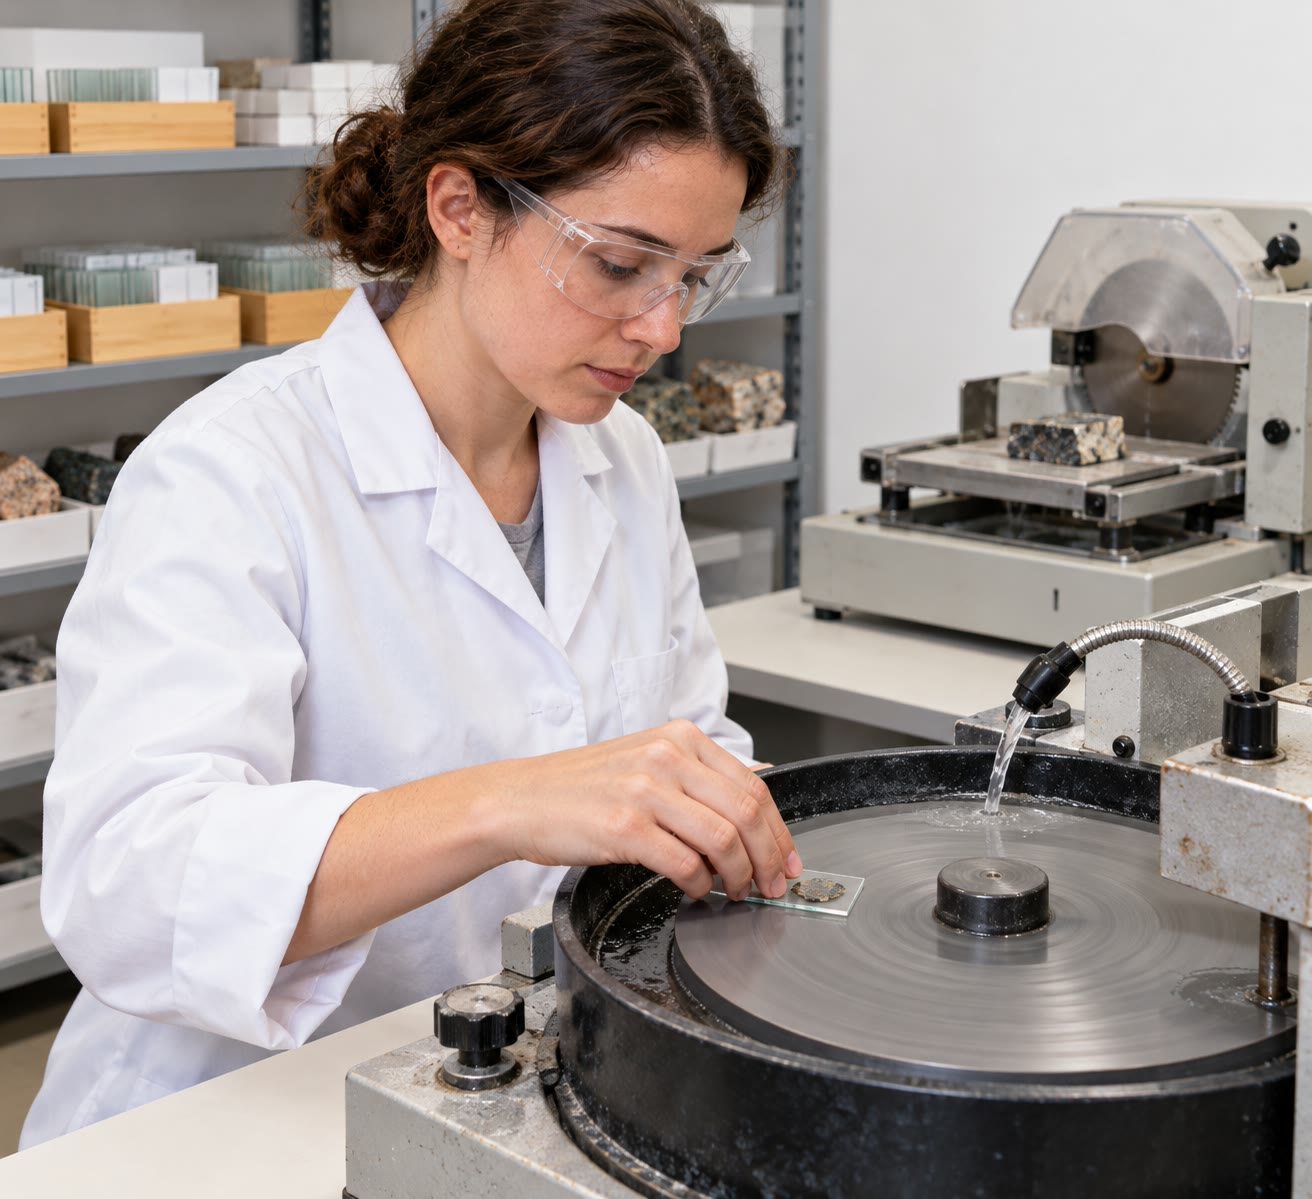
\includegraphics[width=\linewidth]{images/book3/ai/b1-thin-section-lab.jpg}
\end{minipage}
\end{inthelab}

O estudo da lâmina é feito com um microscópio equipado com dois filtros polarizadores. A polarização linear é assunto da física: aqui basta que um filtro polarizador deixe passar apenas a luz que vibra em uma \omterm{def:b1:geological-maps:attitude}{direção}, e que dois filtros colocados em ângulo reto não deixem passar nada.

\begin{definition}[Microscópio de polarização, luz plano-polarizada, polarizadores cruzados]\label{def:b1:field-lab-methods-1:microscope}
Um \emph{microscópio de polarização}\index{microscópio de polarização} é um microscópio de luz transmitida com um filtro polarizador (o polarizador) abaixo de uma platina que gira através de \ang{360} sobre uma escala graduada, e um segundo filtro polarizador (o analisador) entre a objetiva e a ocular, que pode ser movido para dentro ou para fora do caminho da luz, com a sua direção de vibração em ângulo reto com a do polarizador. Com o analisador para fora, a amostra é vista em \emph{luz plano-polarizada}\index{luz plano-polarizada}; com o analisador para dentro, ela é vista entre \emph{polarizadores cruzados}\index{polarizadores cruzados}.
\end{definition}

\begin{omfigure}
\begin{tikzpicture}[font=\scriptsize, x=1cm, y=0.62cm]
\def\comp#1#2#3{\draw[fill=#3] (-1.1,#1-0.18) rectangle (1.1,#1+0.18); \node[right] at (1.3,#1) {#2};}
\draw[omThm!60, line width=3pt, -{Stealth[length=3mm]}] (0,0.3) -- (0,10.6);
\draw[fill=yellow!40] (0,0) circle (0.3); \node[right] at (1.3,0) {lâmpada};
\comp{1.3}{polarizador: transmite uma direção de vibração}{omDef!25}
\draw[omDef, thick, <->] (-0.5,1.3) -- (0.5,1.3);
\draw[fill=white] (-1.0,2.3) .. controls (0,2.75) .. (1.0,2.3) .. controls (0,1.85) .. (-1.0,2.3);
\node[right] at (1.3,2.3) {condensador};
\draw[fill=black!70] (-1.6,3.4) rectangle (1.6,3.55);
\draw[fill=icsJurassic!40] (-0.5,3.55) rectangle (0.5,3.65);
\node[right] at (1.7,3.48) {platina giratória, graduada em graus, com a lâmina};
\draw[fill=white] (-0.45,4.5) rectangle (0.45,5.4); \node[right] at (1.3,4.95) {objetiva};
\comp{6.2}{fenda para acessórios}{black!10}
\comp{7.2}{analisador: dentro (polarizadores cruzados) ou fora (luz plano-polarizada)}{omDef!25}
\draw[omDef, thick, <->] (0,6.85) -- (0,7.55);
\comp{8.2}{lente de Bertrand (opcional)}{black!5}
\draw[fill=white] (-0.35,9.1) rectangle (0.35,10.0); \node[right] at (1.3,9.55) {ocular com retículo};
\end{tikzpicture}

{\small O caminho da luz de um \omterm{def:b1:field-lab-methods-1:microscope}{microscópio de polarização} (esquemático, de baixo para cima). O polarizador e o analisador vibram em ângulo reto (setas duplas); com nada entre eles, os \omterm{def:b1:field-lab-methods-1:microscope}{polarizadores cruzados} dão um campo preto.}
\end{omfigure}

Entre \omterm{def:b1:field-lab-methods-1:microscope}{polarizadores cruzados}, o vidro da lâmina, a resina e qualquer mineral isotrópico (cujas propriedades ópticas são as mesmas em todas as direções, como nos cristais cúbicos) permanecem pretos, qualquer que seja a rotação da platina. A maioria dos minerais não é isotrópica: eles alteram a polarização da luz que os atravessa e aparecem em cores de interferência que mudam quando a platina gira, e se extinguem quatro vezes em uma volta completa. Por que o fazem, e como as cores e os ângulos identificam um mineral, é o assunto de \cref{ch:b1:optical-mineralogy}. Os minerais em \omterm{def:b1:field-lab-methods-1:thin-section}{lâmina delgada} costumam ser examinados em aumentos de cerca de $16\times$ a $400\times$.
% ledger: jaic:magnification

\begin{omfigure}
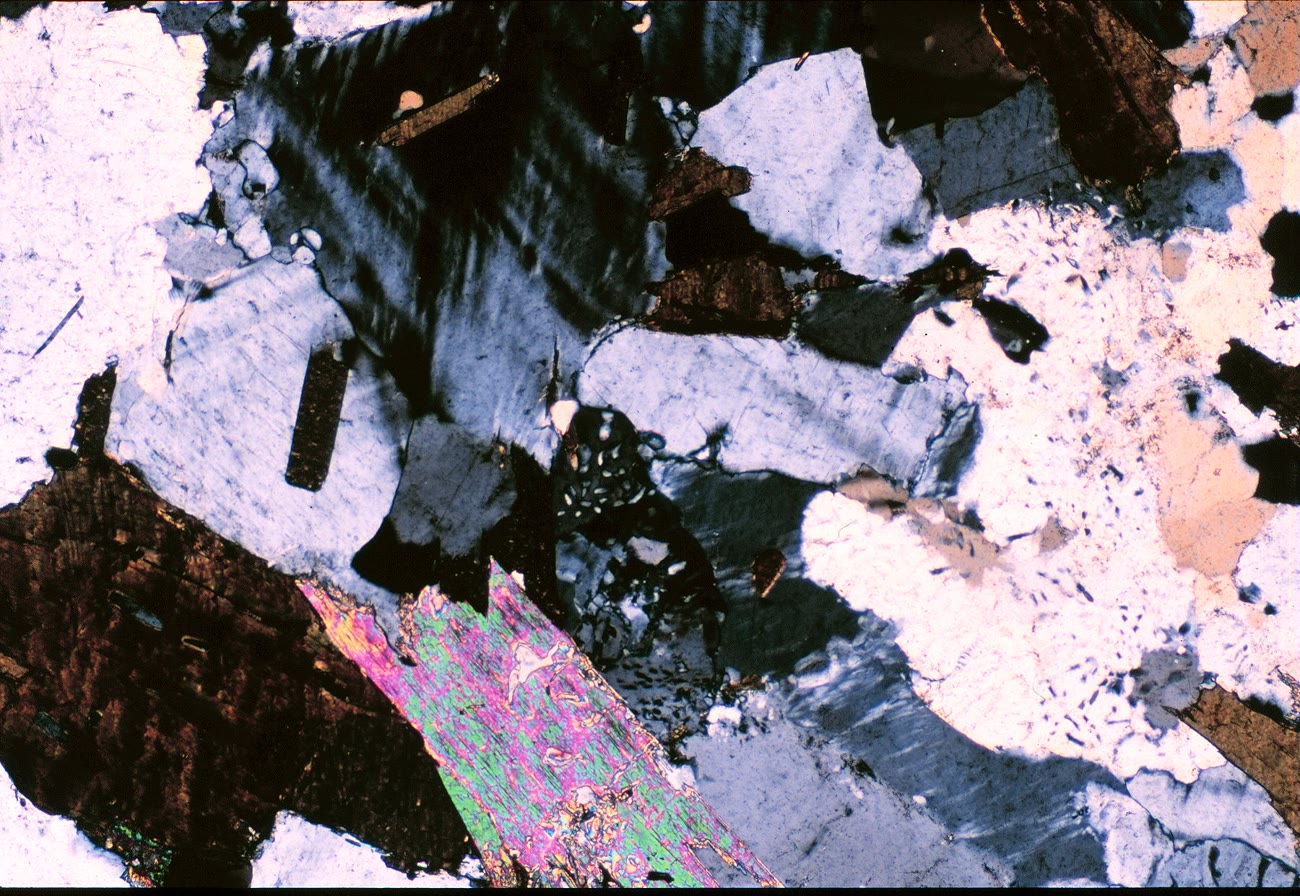
\includegraphics[width=0.55\linewidth]{images/book3/b1-granite-thin-section-xpl.jpg}
% ledger: commons:granite-xpl

{\small Um granito em \omterm{def:b1:field-lab-methods-1:thin-section}{lâmina delgada} entre \omterm{def:b1:field-lab-methods-1:microscope}{polarizadores cruzados}. A biotita é marrom, a muscovita mostra cores de interferência rosa e verdes vivas, o plagioclásio é listrado pelas suas maclas, e o quartzo é branco a cinza. Fotografia de Darla Sondrol, CC0 (Wikimedia Commons).}
\end{omfigure}

\begin{safety}
O trabalho de campo e de laboratório é tornado seguro por regras profissionais, não pela sorte. No campo, os geólogos trabalham em duplas ou deixam um plano escrito do seu percurso e da hora de retorno; levam previsões do tempo, mapas e primeiros socorros, mantêm-se afastados do pé e da borda de falésias e de frentes de pedreira, e usam capacete e proteção para os olhos onde a rocha pode cair ou se estilhaçar; o trabalho em sítios ativos segue as regras do operador. No laboratório, serras e politrizes funcionam protegidas por guardas, com água para conter a poeira; resinas e ácidos são manipulados com luvas e óculos sob exaustão, e cada produto químico tem a sua ficha de segurança. Nenhuma dessas atividades é para um leitor deste livro somente: o capítulo descreve a prática profissional.
\end{safety}

\section{Exercícios}

\begin{exercise}[$\star$]\label{exo:b1:field-lab-methods-1:1}
Um receptor de satélite dá posições com cerca de \qty{4.9}{m} de erro. Quanto isso representa num mapa na escala 1:10\,000? E na escala 1:25\,000?
\end{exercise}

\begin{exercise}[$\star$]\label{exo:b1:field-lab-methods-1:2}
Uma bússola sem ajuste de declinação lê no estrato o \omterm{def:b1:geological-maps:attitude}{sentido de mergulho} \ang{052}. Dê o \omterm{def:b1:geological-maps:attitude}{sentido de mergulho} geográfico se a leitura foi feita em Reykjavik em 1º de janeiro de 2026, e depois em Wellington no mesmo dia (caixa datada).
\end{exercise}

\begin{exercise}[$\star$]\label{exo:b1:field-lab-methods-1:3}
Um \omterm{def:b1:geological-maps:fold}{eixo de dobra} cai \ang{20} em direção a \ang{015}. Escreva a sua orientação como no texto e dê o seu vetor unitário para baixo em componentes leste, norte e cima.
\end{exercise}

\begin{exercise}[$\star$]\label{exo:b1:field-lab-methods-1:4}
Três leituras de uma junta vertical dão os \omterm{def:b1:spherical-astronomy:horizontal}{azimutes} da sua normal \ang{350}, \ang{358} e \ang{006}. Calcule a sua média aritmética e, depois, o \omterm{def:b1:spherical-astronomy:horizontal}{azimute} da soma dos três vetores unitários horizontais. Qual média é a correta?
\end{exercise}

\begin{exercise}[$\star\star$]\label{exo:b1:field-lab-methods-1:5}
Cinco leituras do \omterm{def:b1:geological-maps:attitude}{mergulho} de um mesmo estrato são \ang{34}, \ang{37}, \ang{35}, \ang{33} e \ang{36}. Calcule a sua média, o seu desvio padrão e o erro padrão da média.
\end{exercise}

\begin{exercise}[$\star\star$]\label{exo:b1:field-lab-methods-1:6}
Um geólogo faz a média de uma leitura em cada flanco de uma \omterm{def:b1:geological-maps:fold}{dobra} simétrica: $090/30$ e $270/30$. Calcule a média vetorial e $\bar R$. O que deu errado?
\end{exercise}

\begin{exercise}[$\star\star$]\label{exo:b1:field-lab-methods-1:7}
Estrias em uma superfície de acamamento de \omterm{def:b1:geological-maps:attitude}{atitude} $080/12$ têm \omterm{def:b1:field-lab-methods-1:trend-plunge}{rumo} \ang{120}. Qual é o seu \omterm{def:b1:field-lab-methods-1:trend-plunge}{caimento}? Qual seria para o \omterm{def:b1:field-lab-methods-1:trend-plunge}{rumo} \ang{170}?
\end{exercise}

\begin{exercise}[$\star\star$]\label{exo:b1:field-lab-methods-1:8}
Em Edimburgo a declinação magnética é \ang{-0.47} em 1º de janeiro de 2026 e varia \ang{+0.20} por ano. Supondo que a variação se mantenha constante, quando ela se anula, e qual é o seu valor em 1º de janeiro de 2030?
\end{exercise}

\begin{exercise}[$\star\star$]\label{exo:b1:field-lab-methods-1:9}
Três leituras de um mesmo estrato são $080/10$, $080/12$ e $080/14$. Mostre que a sua média vetorial é $080/12$, calcule $\bar R$ e a estimativa $\sqrt{2(1 - \bar R)}$ de $\theta_{\text{rms}}$, e compare-a com o ângulo quadrático médio exato.
\end{exercise}

\begin{exercise}[$\star\star\star$]\label{exo:b1:field-lab-methods-1:10}
Uma \omterm{def:b1:field-lab-methods-1:thin-section}{lâmina delgada} corta um grão esférico de raio $r$ a uma distância $h$ do seu centro, com $h$ igualmente provável em qualquer ponto entre 0 e $r$. Mostre que o raio médio do círculo visto na seção é $\pi r/4$. Grãos de quartzo com \qty{0.50}{mm} de diâmetro aparecem, em média, com que tamanho em \omterm{def:b1:field-lab-methods-1:thin-section}{lâmina delgada}?
\end{exercise}

\begin{exercise}[$\star\star\star$]\label{exo:b1:field-lab-methods-1:11}
Mostre que, se cada \omterm{def:b1:geological-maps:attitude}{sentido de mergulho} de um conjunto de leituras é aumentado do mesmo ângulo $D$, o \omterm{def:b1:geological-maps:attitude}{sentido de mergulho} da sua média vetorial aumenta de $D$, e o seu \omterm{def:b1:geological-maps:attitude}{mergulho} não muda. Por que isso importa para a correção da declinação?
\end{exercise}

\begin{exercise}[$\star\star\star$]\label{exo:b1:field-lab-methods-1:12}
Em um estrato que mergulha \ang{12}, a normal de uma leitura única se dispersa com desvio padrão de \ang{2} em cada uma de duas direções perpendiculares: ao longo da linha de maior \omterm{def:b1:geological-maps:attitude}{mergulho}, o que muda o \omterm{def:b1:geological-maps:attitude}{mergulho}, e através dela, o que muda o \omterm{def:b1:geological-maps:attitude}{sentido de mergulho}. Quantas leituras são necessárias para um erro padrão de \ang{0.5} no \omterm{def:b1:geological-maps:attitude}{mergulho} médio? E de \ang{1} no \omterm{def:b1:geological-maps:attitude}{sentido de mergulho} médio?
\end{exercise}

\section{Problema: uma temporada de campo no flanco leste de Varden}

\begin{problem}[{Problema de fim de semana --- média de doze leituras de bússola, medida da sua dispersão, correção delas e comparação com as sondagens}]
\label{pb:b1:field-lab-methods-1:1}
% readings: figdata/bachelor-1/attitude_stats.py (part normals); values: calc/ch06.py
Um geólogo mediu a estratificação do flanco leste do \omterm{def:b1:geological-maps:fold}{anticlinal} de Varden em doze estações, com a bússola ajustada para a declinação, arredondando ao grau. A tabela dá cada leitura (\omterm{def:b1:geological-maps:attitude}{sentido de mergulho}/\omterm{def:b1:geological-maps:attitude}{mergulho}) e as componentes de sua normal unitária para cima $\vec n = (n_E, n_N, n_U)$, arredondadas a quatro casas decimais.
\begin{center}
\small
\begin{tabular}{rcccc@{\qquad}rcccc}
\hline
 & leitura & $n_E$ & $n_N$ & $n_U$ & & leitura & $n_E$ & $n_N$ & $n_U$ \\
\hline
1 & $076/11$ & 0.1851 & 0.0462 & 0.9816 & 7 & $083/11$ & 0.1894 & 0.0233 & 0.9816 \\
2 & $081/13$ & 0.2222 & 0.0352 & 0.9744 & 8 & $083/12$ & 0.2064 & 0.0253 & 0.9781 \\
3 & $078/16$ & 0.2696 & 0.0573 & 0.9613 & 9 & $085/12$ & 0.2071 & 0.0181 & 0.9781 \\
4 & $081/11$ & 0.1885 & 0.0298 & 0.9816 & 10 & $078/11$ & 0.1866 & 0.0397 & 0.9816 \\
5 & $076/10$ & 0.1685 & 0.0420 & 0.9848 & 11 & $081/13$ & & & \\
6 & $083/14$ & 0.2401 & 0.0295 & 0.9703 & 12 & $082/11$ & & & \\
\hline
\end{tabular}
\end{center}

\medskip
\noindent\textbf{Parte I --- A atitude média.}
\begin{enumerate}
  \item Calcule as médias aritméticas dos doze \omterm{def:b1:geological-maps:attitude}{sentidos de mergulho} e dos doze \omterm{def:b1:geological-maps:attitude}{mergulhos}.
  \item Dê um exemplo de duas leituras para as quais a média aritmética dos \omterm{def:b1:geological-maps:attitude}{sentidos de mergulho} é absurda, e diga por que ela é segura aqui.
  \item Mostre que $\vec n = (\sin\delta\sin\alpha, \sin\delta\cos\alpha,
        \cos\delta)$ é um vetor unitário perpendicular à linha de \omterm{def:b1:geological-maps:attitude}{mergulho} e à
        linha de \omterm{def:b1:geological-maps:attitude}{direção} do plano $\alpha/\delta$.
  \item Complete a tabela para as leituras 11 e 12.
  \item Calcule a resultante $\vec S$ das doze normais.
  \item Calcule $\|\vec S\|$ e o comprimento médio da resultante $\bar R$.
  \item Deduza a média vetorial: o seu \omterm{def:b1:geological-maps:attitude}{sentido de mergulho} e o seu \omterm{def:b1:geological-maps:attitude}{mergulho}.
\end{enumerate}

\medskip
\noindent\textbf{Parte II --- A dispersão.}
\begin{enumerate}[resume]
  \item Calcule os desvios padrão amostrais dos \omterm{def:b1:geological-maps:attitude}{sentidos de mergulho} e dos \omterm{def:b1:geological-maps:attitude}{mergulhos}.
  \item Usando \cref{prop:b1:field-lab-methods-1:vector-mean}, estime o ângulo quadrático médio $\theta_{\text{rms}}$ entre as leituras e a sua média, em graus.
  \item Preveja $\theta_{\text{rms}}$ a partir dos dois desvios padrão da questão 8 e da fórmula de erro do capítulo, e compare.
  \item Qual dos dois desvios padrão contribui mais para $\theta_{\text{rms}}$, e por quê?
  \item Calcule os erros padrão do \omterm{def:b1:geological-maps:attitude}{mergulho} médio e do \omterm{def:b1:geological-maps:attitude}{sentido de mergulho} médio.
  \item A dispersão dos \omterm{def:b1:geological-maps:attitude}{sentidos de mergulho}, de \ang{2.9}, é sinal de medição descuidada? Explique.
\end{enumerate}

\medskip
\noindent\textbf{Parte III --- A declinação.}
\begin{enumerate}[resume]
  \item Uma segunda geóloga esqueceu de ajustar a declinação. As suas doze leituras têm a média vetorial $083.1/12.1$ em \omterm{def:b1:spherical-astronomy:horizontal}{azimutes} magnéticos. Suponha que a declinação magnética nas Colinas de Varden naquele ano seja de \ang{2.5} para oeste. Qual é a sua média em \omterm{def:b1:spherical-astronomy:horizontal}{azimutes} geográficos?
  \item Por que o seu \omterm{def:b1:geological-maps:attitude}{mergulho} médio está certo sem correção?
  \item Ela poderia ter corrigido cada leitura antes de fazer a média, em vez da média? Isso muda a resposta (\cref{exo:b1:field-lab-methods-1:11})?
  \item Dez anos depois, um estudante reutiliza o ajuste de declinação dela enquanto a declinação mudou \ang{0.2} por ano. Qual é o tamanho do erro, comparado com o erro padrão da questão 12?
  \item Dê a \omterm{def:b1:geological-maps:attitude}{direção} da \omterm{def:b1:geological-maps:attitude}{atitude} média do primeiro geólogo pela regra da mão direita.
\end{enumerate}

\medskip
\noindent\textbf{Parte IV --- Bússola e sondagens.}
\begin{enumerate}[resume]
  \item A partir de três sondagens, \cref{ch:b1:geological-maps} encontrou para a base do calcário a \omterm{def:b1:geological-maps:attitude}{atitude} $080.6/12.2$. Compare-a com a média vetorial da questão 7, ângulo a ângulo.
  \item Calcule o ângulo entre as duas normais.
  \item O erro padrão da \omterm{def:b1:geological-maps:attitude}{direção} média é cerca de $\theta_{\text{rms}}/\sqrt N$. A diferença da questão 20 é significativa?
  \item Quantas leituras reduziriam esse erro padrão à metade?
  \item Cite dois erros que nenhum número de leituras reduziria.
  \item Dê a \omterm{def:b1:geological-maps:attitude}{atitude} média do flanco leste a partir das doze leituras, na forma \omterm{def:b1:geological-maps:attitude}{sentido de mergulho}/\omterm{def:b1:geological-maps:attitude}{mergulho} arredondada ao grau.
\end{enumerate}
\end{problem}
